In diesem Kapitel werden die Messergebnisse vorgestellt, die eine
Charakterisierung des Lasersystems erlauben. Dabei werden zunächst Messungen
aufgeführt, die die reine Frequenzstabilität der Laser beschreiben. Dazu werden
Lang- und Kurzzeitverhalten sowohl des alten als auch den neuen Lasersystems
untersucht (Abschn. \ref{sec:laserstabilitaet}). Weiterhin wird das
Linearitätsverhalten der \textit{iScans} charakterisiert, wobei die
Nichtlinearitäten und deren Auswirkung auf die
Frequenzverstimmungsroutine gemessen werden (Abschn.
\ref{sec:linearisierung}). Abschnitt \ref{spektroskopie_an_uran} beschäftigt
sich mit den bishereigen spektroskopischen Messungen an Uran mit dem alten und
neuen System, dem bisher verwendeten Anregungsschema und der Suche nach neuen
Anregungsschemata. In Abschn. \ref{sec:countraten_fluktuation} wird kurz auf die
Gesamtstabilität der Systeme eingegangen und Countratenfluktuationen vorgstellt.
Zu Beginn dieses Kapitels soll allerdings noch eine Charakterisierung des
verwendeten FPIs besprochen werden.

\section{Charakterisierung des FPIs}\label{sec:charakterisierung_FPI}
Im Folgenden sollen die gemessenen Charakteristiken wie FSR und Finesse des FPIs
vorgestellt werden.

\subsection{FSR}\label{subsec:FSR-messung}
Um korrekte Relativfrequenzen berechnen und anfahren zu
können, ist von essenzieller Wichtigkeit, den FSR des FPIs möglichst genau zu kennen. Um
frequenzabhängige optische Elemente zu eichen, wird immer eine bzw. mehrere
Referenzfrequnez(en) benötigt, die wiederum nur bis auf eine endliche
Genauigkeit bestimmt werden kann/können. Das FPI kann auf verschiedene
Weise geeicht werden.\par
Eine in der Arbeit \cite{kuschnick:2000:diplomarbeit}
vorgestellte Methode bedient sich der Hyperfeinstrukturübergänge des
Cäsiumatoms, für die sehr genaue Literaturwerte mit Fehlern von wenigen KHz \cite{PhysRevA.38.1616} bekannt sind
und als absolute Relativfrequenzen dienen können. Der damals gemessene FSR wurde
mit einer Genauigkeit von $6,7\cdot10^{-6}$ bzw. $4,0\cdot10^{-5}$ bestimmt. Da
diese Methode eines hohen experimentellen Aufwands bedarf, wurde hier
eine andere sog. \textit{Nonius-Methode} angewandt, welche bereits im Rahmen der
Arbeit \cite{schumann:2005:dissertation} zum Einsatz kam. Hierbei werden eine
Reihe von Absolutfrequenzen eines Lasers mit dem Wavemeter gemessen, für die das
FPI transmittiv ist. Schnell zu realisieren ist dies durch Verfahren eines
Laser-Fringes auf den He:Ne-Fringe. Die Relativfrequenzen sind also ganzzahlige
Vielfache eines FSRs. Idee ist es nun, den Wert für den FSR zu finden, der alle
Relativfrequenzen möglichst ganzzahlig teilt. Das Minimum der Fehlerfunktion
\begin{equation}\label{eq:nonius}
	f(\text{FSR})=\sum\limits_i\left[\frac{\delta\nu_i}{\text{FSR}}-\text{Round}\left(\frac{\delta\nu_i}{\text{FSR}}\right)\right]^2\,.
\end{equation}
ist ein gutes Maß für den wahrscheinlichsten FSR.
Ein Summand besteht aus einer Aneinanderreihung von Parabeln, deren Minima bei
$\nicefrac{\text{FSR}_{wahr}}{n}$ mit $n\in\N$ liegen, wobei $\text{FSR}_{wahr}$
der tatsächliche FSR ist. Es ist wichtig, sowohl große als auch kleine
Relativfrequenzen zu messen, damit sowohl in kleinen als auch in großen
Frequenzbereichen die Mehrdeutigkeit eliminiert wird, was sich durch Vergrößern
der Relativfrequenz mit einem konstanten Faktor erreichen lässt:
\begin{equation}\label{eq:nonius_faktor}
	\nu_i=a\cdot\nu_{i-1}\,.
\end{equation}
Weiterhin ist darauf zu achten, dass dieser Faktor maximal in der Größenordnung
des Verhältnisses
\begin{equation}\label{eq:nonius_faktor}
	a\stackrel{!}{<}\frac{\text{FSR}}{2\Delta\nu}\,,
\end{equation}
liegt, wobei $\Delta\nu$ der Fehler des Wavemeters ($40\,$MHz) ist, da sonst
mehrere Minima von Summanden höherer Relativfrequenzen in einem Minimum
eines Summanden einer kleineren Relativfrequenz liegen. Das würde eine
Eindeutige Aussage über den wahren FSR erschweren. Da bei
einem Faktor $a=3$ große Probleme bei der eindeutigen Bestimmung des FSR
aufgetreten sind, wurden einige Simulationen mit \textit{Mathematica}
durchgeführt, die bei der Optimierung dieses Parameters geholfen haben.
In Anhang \ref{anh:sec:nonius_simulationen} finden sich Simulationen für einige
Relativfrequenzen und verschiedene Werte von $a$. Wie man sieht, eignet sich
$a=2$ gut zur eindeutigen FSR-Bestimmung.\par
\begin{table}[h]
	%Summe der Breiten muss 0.91 mal \textwidth sein.
	\begin{tabular}{R{0.05\textwidth}R{0.15\textwidth}R{0.10\textwidth}R{0.31\textwidth}R{0.30\textwidth}}
		\toprule
		\multicolumn{1}{C{0.05\textwidth}}{i} &
		\multicolumn{1}{C{0.15\textwidth}}{$\nu$ [MHz]} &
		\multicolumn{1}{C{0.10\textwidth}}{T [°C]} &
		\multicolumn{1}{C{0.25\textwidth}}{ungefähre Verstimmung zum
		Schritt i-1 [GHz]} &
		\multicolumn{1}{C{0.23\textwidth}}{ungefähre FSR-Anzahl}\\
		\midrule[1px]
		\hline
		%%%%%%%%%%%%%%%%%%%%%%%%%%%%%%%%%%%%%%%%%%%%%%%%%%%%%%%%%%%%%%%%%%%%%%
%%                                                                  %%
%%  This is a LaTeX2e table fragment exported from Gnumeric.        %%
%%                                                                  %%
%%%%%%%%%%%%%%%%%%%%%%%%%%%%%%%%%%%%%%%%%%%%%%%%%%%%%%%%%%%%%%%%%%%%%%
%i	&nu [Mhz]	&T [°C]	&ungefähre Verstimmung zum vorherigen Schritt [Ghz]
% &ungefähre Anzahl von FSR\\
0	&376580060	&23,0	&0	&0\\
1	&376580330	&23,1	&0,3	&1\\
2	&376580950	&23,0	&0,6	&2\\
3	&376582120	&23,1	&1,2	&4\\
4	&376584550	&23,1	&2,4	&8\\
5	&376589310	&23,1	&4,8	&16\\
6	&376598860	&23,1	&9,6	&32\\
7	&376618200	&23,1	&19,2	&64\\
8	&376656670	&23,1	&38,4	&128\\
9	&376733260	&23,1	&76,8	&256\\
10	&376887090	&23,1	&153,6	&512\\
11	&377194120	&23,1	&307,2	&1024\\
12	&377808470	&23,1	&614,4	&2048\\
13	&379037480	&23,1	&1228,8	&4096\\
14	&381494880	&23,1	&2457,6	&8192\\
15	&386410030	&23,1	&4915,2	&16384\\
16	&396240640	&23,0	&9830,4	&32768\\

		\bottomrule[1px]
	\end{tabular}
	\caption[FSR Messung]{Aufgelistet sind die Messwerte für die Bestimmung des
	FSRs des FPIs. Messdatum: 14.01.2012, 1:30 Uhr}
	\label{tab:nonius_FSR_messung}
\end{table}
Dafür wurden die in Tab. \ref{tab:nonius_FSR_messung} aufgelisteten Frequenzen
mit dem Diodenlaser \textit{TA-Pro} von \textit{Toptica} gemessen, welcher sich
von $745\,$nm bis $795\,$nm mühelos durchstimmen lässt.
Die Temperatur unterlag Schwankungen von $\pm0,1\,$K, was nach
\cite{kuschnick:2000:diplomarbeit} im Sub-KHz-Bereich liegt.
Abbildung \ref{fig:nonius_FSR_messung} zeigt die Fehlerfunktion für die
gemessenen Frequenzen, wobei alle möglichen $136$ Relativfrequenzen berechnet
wurden. Erfreulicherweise ist ein globales Minimum eindeutig zu identifizieren.
Vergrößert man den Bereich des vermuteten FSRs, findet man über numerische
Methoden
\begin{equation}\label{eq:FSR_messung}
	\text{FSR}=(298,0856\pm0,0026)\,\text{MHz}\,,
\end{equation}
wobei der Fehler durch die halbe Halbwertsbreite der Parabel in Abb.
\ref{subfig:nonius_FSR_messung_d} abgeschätzt werden kann. Daraus folgt ein
relativer Fehler von auf $8,7\cdot10^{-6}$. Ein Aufkleber auf dem FPI von
07.06.1999 gibt an, dass ein FSR von $298,085\pm0,017\,$MHz gemessen wurde.
Sollte dieser Aufkleber eine damalige Messung repräsentieren, stimmt der
14.01.2012 gemessene Wert unter Einbezug der Fehlertoleranz sehr gut mit dem
damaligen Wert überein. Der FSR hat sich nahezu nicht verändert und konnte um
einen Faktor $6,5$ genauer bestimmt werden.
\begin{figure}[H]
 	\centering
 	\fbox{\parbox{\dimexpr \linewidth - 2\fboxrule - 2\fboxsep}{
 	\subfigure[]{
		\label{subfig:nonius_FSR_messung_a}
		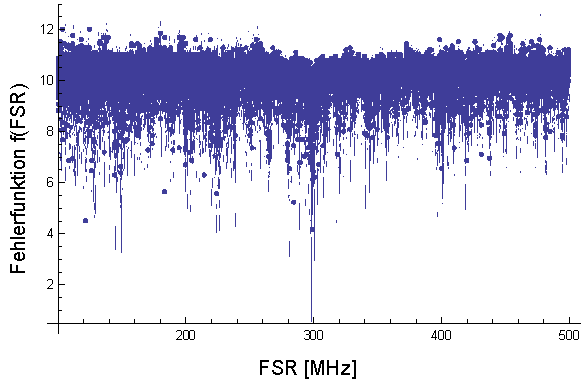
\includegraphics[width=(\textwidth-0.6cm)/2]{plt/nonius_FSR_messung_a}
		}
 	\subfigure[]{
		\label{subfig:nonius_FSR_messung_b}
		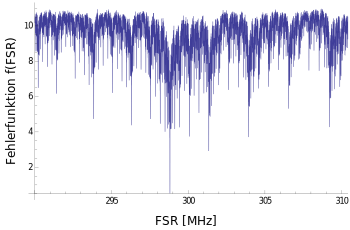
\includegraphics[width=(\textwidth-0.6cm)/2]{plt/nonius_FSR_messung_b}
		}
	 \subfigure[]{
		\label{subfig:nonius_FSR_messung_c}
		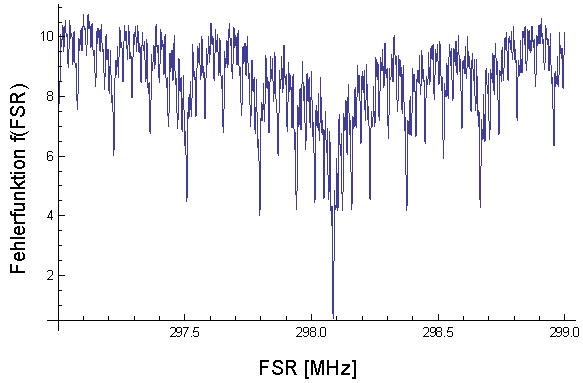
\includegraphics[width=(\textwidth-0.6cm)/2]{plt/nonius_FSR_messung_c}
		}
	\subfigure[]{
		\label{subfig:nonius_FSR_messung_d}
		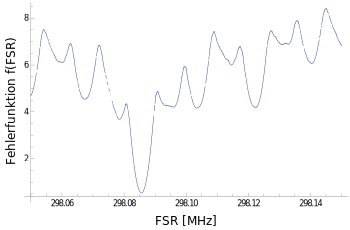
\includegraphics[width=(\textwidth-0.6cm)/2]{plt/nonius_FSR_messung_d}
		}
	}}
	\caption[FSR-Bestimmung]{Die Abbildung zeigt die Plots der Fehlerfunktionen.
	Von (a) nach (d) wurde der Ausschnitt des interessanten Minimums vergrößert. Die
	Stelle des Minimums ist der vermutliche FSR des FPIs.}
	\label{fig:nonius_FSR_messung}
\end{figure}

\subsection{Finesse}\label{subsec:finesse}
In diesem Abschnitt sollen kurz die Messungen der Finesse des FPIs
durchgesprochen werden. Im Gegensatz zum FSR ist die Finesse ein weniger
kritischer Parameter, sollte dennoch groß genug sein, damit die Spitze der
Transmissionsfringes genau mit der FOL-Technik präzise detektiert werden
kann. Wie in Abschn. \ref{subsec:fabry-perot-interferometer} erklärt, ist
die Finesse abhängig von der Wellenlänge des Laserlichts. Deshalb wurde für jeden
Wellenlängenbereich der in diesem System verwendenen Laser die Finesse
gemssen. Dazu wurde jeweils mithilfe eines Oszilloskops das Fringepattern der
steigenden Rampe aufgenommen und daran eine Airy-Funktion
\begin{equation}\label{eq:finesse_messung_01}
	U(t,\kappa,a,b,c) = b\cdot\frac{1}{1+\kappa \sin^2{(at)}}+c
\end{equation}
gefittet, wobei $U$ die verstärkte Spannung an der Photodiode, $t$ die Zeit,
$\kappa$ das Maß für die Finesse und $a$, $b$, $c$ Normierungsgrößen sind.
Abbildung \ref{fig:finesse_messung} zeigt die Plots inklusive Fits der
Fringepattern von \textit{DL-Pro} mit $772\,$nm (a), He:Ne-Laser mit $633\,$nm (b), und dem
blauen Diodenlaser mit $405\,$nm (c).

\begin{figure}[hp]
 	\centering
 	\footnotesize
 	\fbox{\parbox{\dimexpr \linewidth - 2\fboxrule - 2\fboxsep}{
 	\subfigure[]{
		\label{subfig:finesse_messung_a}
		% GNUPLOT: LaTeX picture with Postscript
\begingroup
  \makeatletter
  \providecommand\color[2][]{%
    \GenericError{(gnuplot) \space\space\space\@spaces}{%
      Package color not loaded in conjunction with
      terminal option `colourtext'%
    }{See the gnuplot documentation for explanation.%
    }{Either use 'blacktext' in gnuplot or load the package
      color.sty in LaTeX.}%
    \renewcommand\color[2][]{}%
  }%
  \providecommand\includegraphics[2][]{%
    \GenericError{(gnuplot) \space\space\space\@spaces}{%
      Package graphicx or graphics not loaded%
    }{See the gnuplot documentation for explanation.%
    }{The gnuplot epslatex terminal needs graphicx.sty or graphics.sty.}%
    \renewcommand\includegraphics[2][]{}%
  }%
  \providecommand\rotatebox[2]{#2}%
  \@ifundefined{ifGPcolor}{%
    \newif\ifGPcolor
    \GPcolortrue
  }{}%
  \@ifundefined{ifGPblacktext}{%
    \newif\ifGPblacktext
    \GPblacktexttrue
  }{}%
  % define a \g@addto@macro without @ in the name:
  \let\gplgaddtomacro\g@addto@macro
  % define empty templates for all commands taking text:
  \gdef\gplbacktext{}%
  \gdef\gplfronttext{}%
  \makeatother
  \ifGPblacktext
    % no textcolor at all
    \def\colorrgb#1{}%
    \def\colorgray#1{}%
  \else
    % gray or color?
    \ifGPcolor
      \def\colorrgb#1{\color[rgb]{#1}}%
      \def\colorgray#1{\color[gray]{#1}}%
      \expandafter\def\csname LTw\endcsname{\color{white}}%
      \expandafter\def\csname LTb\endcsname{\color{black}}%
      \expandafter\def\csname LTa\endcsname{\color{black}}%
      \expandafter\def\csname LT0\endcsname{\color[rgb]{1,0,0}}%
      \expandafter\def\csname LT1\endcsname{\color[rgb]{0,1,0}}%
      \expandafter\def\csname LT2\endcsname{\color[rgb]{0,0,1}}%
      \expandafter\def\csname LT3\endcsname{\color[rgb]{1,0,1}}%
      \expandafter\def\csname LT4\endcsname{\color[rgb]{0,1,1}}%
      \expandafter\def\csname LT5\endcsname{\color[rgb]{1,1,0}}%
      \expandafter\def\csname LT6\endcsname{\color[rgb]{0,0,0}}%
      \expandafter\def\csname LT7\endcsname{\color[rgb]{1,0.3,0}}%
      \expandafter\def\csname LT8\endcsname{\color[rgb]{0.5,0.5,0.5}}%
    \else
      % gray
      \def\colorrgb#1{\color{black}}%
      \def\colorgray#1{\color[gray]{#1}}%
      \expandafter\def\csname LTw\endcsname{\color{white}}%
      \expandafter\def\csname LTb\endcsname{\color{black}}%
      \expandafter\def\csname LTa\endcsname{\color{black}}%
      \expandafter\def\csname LT0\endcsname{\color{black}}%
      \expandafter\def\csname LT1\endcsname{\color{black}}%
      \expandafter\def\csname LT2\endcsname{\color{black}}%
      \expandafter\def\csname LT3\endcsname{\color{black}}%
      \expandafter\def\csname LT4\endcsname{\color{black}}%
      \expandafter\def\csname LT5\endcsname{\color{black}}%
      \expandafter\def\csname LT6\endcsname{\color{black}}%
      \expandafter\def\csname LT7\endcsname{\color{black}}%
      \expandafter\def\csname LT8\endcsname{\color{black}}%
    \fi
  \fi
  \setlength{\unitlength}{0.0500bp}%
  \begin{picture}(7936.00,3968.00)%
    \gplgaddtomacro\gplbacktext{%
      \csname LTb\endcsname%
      \put(980,640){\makebox(0,0)[r]{\strut{} 0}}%
      \put(980,983){\makebox(0,0)[r]{\strut{} 0.01}}%
      \put(980,1326){\makebox(0,0)[r]{\strut{} 0.02}}%
      \put(980,1669){\makebox(0,0)[r]{\strut{} 0.03}}%
      \put(980,2012){\makebox(0,0)[r]{\strut{} 0.04}}%
      \put(980,2355){\makebox(0,0)[r]{\strut{} 0.05}}%
      \put(980,2698){\makebox(0,0)[r]{\strut{} 0.06}}%
      \put(980,3041){\makebox(0,0)[r]{\strut{} 0.07}}%
      \put(980,3384){\makebox(0,0)[r]{\strut{} 0.08}}%
      \put(980,3727){\makebox(0,0)[r]{\strut{} 0.09}}%
      \put(1100,440){\makebox(0,0){\strut{}-6}}%
      \put(1909,440){\makebox(0,0){\strut{}-5}}%
      \put(2719,440){\makebox(0,0){\strut{}-4}}%
      \put(3528,440){\makebox(0,0){\strut{}-3}}%
      \put(4338,440){\makebox(0,0){\strut{}-2}}%
      \put(5147,440){\makebox(0,0){\strut{}-1}}%
      \put(5956,440){\makebox(0,0){\strut{} 0}}%
      \put(6766,440){\makebox(0,0){\strut{} 1}}%
      \put(7575,440){\makebox(0,0){\strut{} 2}}%
      \put(160,2183){\rotatebox{-270}{\makebox(0,0){\strut{}Amplitude U [V]}}}%
      \put(4337,140){\makebox(0,0){\strut{}Zeit t [ms]}}%
      \put(2719,2894){\makebox(0,0)[l]{\strut{}$\kappa = 992\pm14$}}%
      \put(2719,2677){\makebox(0,0)[l]{\strut{}$a = (562.020\pm0.044)\,$s$^{-1}$}}%
      \put(2719,2461){\makebox(0,0)[l]{\strut{}$b = (0.05961\pm0.00028)\,$V}}%
      \put(2719,2245){\makebox(0,0)[l]{\strut{}$c = (0.010994\pm0.000029)\,$V}}%
    }%
    \gplgaddtomacro\gplfronttext{%
      \csname LTb\endcsname%
      \put(6672,3564){\makebox(0,0)[r]{\strut{}Fringepattern}}%
      \csname LTb\endcsname%
      \put(6672,3364){\makebox(0,0)[r]{\strut{}Fit}}%
    }%
    \gplbacktext
    \put(0,0){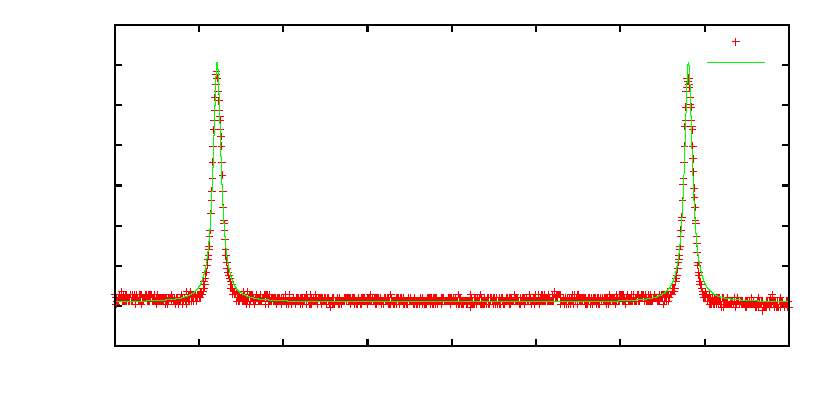
\includegraphics{finesse_messung_a}}%
    \gplfronttext
  \end{picture}%
\endgroup

		}
 	\subfigure[]{
		\label{subfig:finesse_messung_b}
		% GNUPLOT: LaTeX picture with Postscript
\begingroup
  \makeatletter
  \providecommand\color[2][]{%
    \GenericError{(gnuplot) \space\space\space\@spaces}{%
      Package color not loaded in conjunction with
      terminal option `colourtext'%
    }{See the gnuplot documentation for explanation.%
    }{Either use 'blacktext' in gnuplot or load the package
      color.sty in LaTeX.}%
    \renewcommand\color[2][]{}%
  }%
  \providecommand\includegraphics[2][]{%
    \GenericError{(gnuplot) \space\space\space\@spaces}{%
      Package graphicx or graphics not loaded%
    }{See the gnuplot documentation for explanation.%
    }{The gnuplot epslatex terminal needs graphicx.sty or graphics.sty.}%
    \renewcommand\includegraphics[2][]{}%
  }%
  \providecommand\rotatebox[2]{#2}%
  \@ifundefined{ifGPcolor}{%
    \newif\ifGPcolor
    \GPcolortrue
  }{}%
  \@ifundefined{ifGPblacktext}{%
    \newif\ifGPblacktext
    \GPblacktexttrue
  }{}%
  % define a \g@addto@macro without @ in the name:
  \let\gplgaddtomacro\g@addto@macro
  % define empty templates for all commands taking text:
  \gdef\gplbacktext{}%
  \gdef\gplfronttext{}%
  \makeatother
  \ifGPblacktext
    % no textcolor at all
    \def\colorrgb#1{}%
    \def\colorgray#1{}%
  \else
    % gray or color?
    \ifGPcolor
      \def\colorrgb#1{\color[rgb]{#1}}%
      \def\colorgray#1{\color[gray]{#1}}%
      \expandafter\def\csname LTw\endcsname{\color{white}}%
      \expandafter\def\csname LTb\endcsname{\color{black}}%
      \expandafter\def\csname LTa\endcsname{\color{black}}%
      \expandafter\def\csname LT0\endcsname{\color[rgb]{1,0,0}}%
      \expandafter\def\csname LT1\endcsname{\color[rgb]{0,1,0}}%
      \expandafter\def\csname LT2\endcsname{\color[rgb]{0,0,1}}%
      \expandafter\def\csname LT3\endcsname{\color[rgb]{1,0,1}}%
      \expandafter\def\csname LT4\endcsname{\color[rgb]{0,1,1}}%
      \expandafter\def\csname LT5\endcsname{\color[rgb]{1,1,0}}%
      \expandafter\def\csname LT6\endcsname{\color[rgb]{0,0,0}}%
      \expandafter\def\csname LT7\endcsname{\color[rgb]{1,0.3,0}}%
      \expandafter\def\csname LT8\endcsname{\color[rgb]{0.5,0.5,0.5}}%
    \else
      % gray
      \def\colorrgb#1{\color{black}}%
      \def\colorgray#1{\color[gray]{#1}}%
      \expandafter\def\csname LTw\endcsname{\color{white}}%
      \expandafter\def\csname LTb\endcsname{\color{black}}%
      \expandafter\def\csname LTa\endcsname{\color{black}}%
      \expandafter\def\csname LT0\endcsname{\color{black}}%
      \expandafter\def\csname LT1\endcsname{\color{black}}%
      \expandafter\def\csname LT2\endcsname{\color{black}}%
      \expandafter\def\csname LT3\endcsname{\color{black}}%
      \expandafter\def\csname LT4\endcsname{\color{black}}%
      \expandafter\def\csname LT5\endcsname{\color{black}}%
      \expandafter\def\csname LT6\endcsname{\color{black}}%
      \expandafter\def\csname LT7\endcsname{\color{black}}%
      \expandafter\def\csname LT8\endcsname{\color{black}}%
    \fi
  \fi
  \setlength{\unitlength}{0.0500bp}%
  \begin{picture}(7936.00,3968.00)%
    \gplgaddtomacro\gplbacktext{%
      \csname LTb\endcsname%
      \put(860,640){\makebox(0,0)[r]{\strut{}-0.1}}%
      \put(860,1026){\makebox(0,0)[r]{\strut{} 0}}%
      \put(860,1412){\makebox(0,0)[r]{\strut{} 0.1}}%
      \put(860,1798){\makebox(0,0)[r]{\strut{} 0.2}}%
      \put(860,2184){\makebox(0,0)[r]{\strut{} 0.3}}%
      \put(860,2569){\makebox(0,0)[r]{\strut{} 0.4}}%
      \put(860,2955){\makebox(0,0)[r]{\strut{} 0.5}}%
      \put(860,3341){\makebox(0,0)[r]{\strut{} 0.6}}%
      \put(860,3727){\makebox(0,0)[r]{\strut{} 0.7}}%
      \put(980,440){\makebox(0,0){\strut{}-2}}%
      \put(1922,440){\makebox(0,0){\strut{}-1}}%
      \put(2864,440){\makebox(0,0){\strut{} 0}}%
      \put(3806,440){\makebox(0,0){\strut{} 1}}%
      \put(4749,440){\makebox(0,0){\strut{} 2}}%
      \put(5691,440){\makebox(0,0){\strut{} 3}}%
      \put(6633,440){\makebox(0,0){\strut{} 4}}%
      \put(7575,440){\makebox(0,0){\strut{} 5}}%
      \put(160,2183){\rotatebox{-270}{\makebox(0,0){\strut{}Amplitude U [V]}}}%
      \put(4277,140){\makebox(0,0){\strut{}Zeit t [ms]}}%
      \put(2629,2894){\makebox(0,0)[l]{\strut{}$\kappa = 522.6\pm6.9$}}%
      \put(2629,2677){\makebox(0,0)[l]{\strut{}$a = (686.405\pm0.068)\,$s$^{-1}$}}%
      \put(2629,2461){\makebox(0,0)[l]{\strut{}$b = (0.5879\pm0.0026)\,$V}}%
      \put(2629,2245){\makebox(0,0)[l]{\strut{}$c = (-0.02542\pm0.00035)\,$V}}%
    }%
    \gplgaddtomacro\gplfronttext{%
      \csname LTb\endcsname%
      \put(6672,3564){\makebox(0,0)[r]{\strut{}Fringepattern}}%
      \csname LTb\endcsname%
      \put(6672,3364){\makebox(0,0)[r]{\strut{}Fit}}%
    }%
    \gplbacktext
    \put(0,0){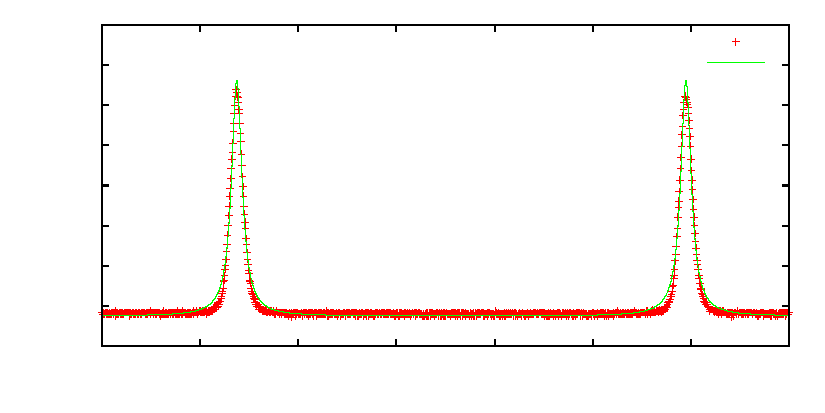
\includegraphics{finesse_messung_b}}%
    \gplfronttext
  \end{picture}%
\endgroup

		}
	 \subfigure[]{
		\label{subfig:finesse_messung_c}
		% GNUPLOT: LaTeX picture with Postscript
\begingroup
  \makeatletter
  \providecommand\color[2][]{%
    \GenericError{(gnuplot) \space\space\space\@spaces}{%
      Package color not loaded in conjunction with
      terminal option `colourtext'%
    }{See the gnuplot documentation for explanation.%
    }{Either use 'blacktext' in gnuplot or load the package
      color.sty in LaTeX.}%
    \renewcommand\color[2][]{}%
  }%
  \providecommand\includegraphics[2][]{%
    \GenericError{(gnuplot) \space\space\space\@spaces}{%
      Package graphicx or graphics not loaded%
    }{See the gnuplot documentation for explanation.%
    }{The gnuplot epslatex terminal needs graphicx.sty or graphics.sty.}%
    \renewcommand\includegraphics[2][]{}%
  }%
  \providecommand\rotatebox[2]{#2}%
  \@ifundefined{ifGPcolor}{%
    \newif\ifGPcolor
    \GPcolortrue
  }{}%
  \@ifundefined{ifGPblacktext}{%
    \newif\ifGPblacktext
    \GPblacktexttrue
  }{}%
  % define a \g@addto@macro without @ in the name:
  \let\gplgaddtomacro\g@addto@macro
  % define empty templates for all commands taking text:
  \gdef\gplbacktext{}%
  \gdef\gplfronttext{}%
  \makeatother
  \ifGPblacktext
    % no textcolor at all
    \def\colorrgb#1{}%
    \def\colorgray#1{}%
  \else
    % gray or color?
    \ifGPcolor
      \def\colorrgb#1{\color[rgb]{#1}}%
      \def\colorgray#1{\color[gray]{#1}}%
      \expandafter\def\csname LTw\endcsname{\color{white}}%
      \expandafter\def\csname LTb\endcsname{\color{black}}%
      \expandafter\def\csname LTa\endcsname{\color{black}}%
      \expandafter\def\csname LT0\endcsname{\color[rgb]{1,0,0}}%
      \expandafter\def\csname LT1\endcsname{\color[rgb]{0,1,0}}%
      \expandafter\def\csname LT2\endcsname{\color[rgb]{0,0,1}}%
      \expandafter\def\csname LT3\endcsname{\color[rgb]{1,0,1}}%
      \expandafter\def\csname LT4\endcsname{\color[rgb]{0,1,1}}%
      \expandafter\def\csname LT5\endcsname{\color[rgb]{1,1,0}}%
      \expandafter\def\csname LT6\endcsname{\color[rgb]{0,0,0}}%
      \expandafter\def\csname LT7\endcsname{\color[rgb]{1,0.3,0}}%
      \expandafter\def\csname LT8\endcsname{\color[rgb]{0.5,0.5,0.5}}%
    \else
      % gray
      \def\colorrgb#1{\color{black}}%
      \def\colorgray#1{\color[gray]{#1}}%
      \expandafter\def\csname LTw\endcsname{\color{white}}%
      \expandafter\def\csname LTb\endcsname{\color{black}}%
      \expandafter\def\csname LTa\endcsname{\color{black}}%
      \expandafter\def\csname LT0\endcsname{\color{black}}%
      \expandafter\def\csname LT1\endcsname{\color{black}}%
      \expandafter\def\csname LT2\endcsname{\color{black}}%
      \expandafter\def\csname LT3\endcsname{\color{black}}%
      \expandafter\def\csname LT4\endcsname{\color{black}}%
      \expandafter\def\csname LT5\endcsname{\color{black}}%
      \expandafter\def\csname LT6\endcsname{\color{black}}%
      \expandafter\def\csname LT7\endcsname{\color{black}}%
      \expandafter\def\csname LT8\endcsname{\color{black}}%
    \fi
  \fi
  \setlength{\unitlength}{0.0500bp}%
  \begin{picture}(7936.00,3968.00)%
    \gplgaddtomacro\gplbacktext{%
      \csname LTb\endcsname%
      \put(860,640){\makebox(0,0)[r]{\strut{} 1}}%
      \put(860,983){\makebox(0,0)[r]{\strut{} 1.5}}%
      \put(860,1326){\makebox(0,0)[r]{\strut{} 2}}%
      \put(860,1669){\makebox(0,0)[r]{\strut{} 2.5}}%
      \put(860,2012){\makebox(0,0)[r]{\strut{} 3}}%
      \put(860,2355){\makebox(0,0)[r]{\strut{} 3.5}}%
      \put(860,2698){\makebox(0,0)[r]{\strut{} 4}}%
      \put(860,3041){\makebox(0,0)[r]{\strut{} 4.5}}%
      \put(860,3384){\makebox(0,0)[r]{\strut{} 5}}%
      \put(860,3727){\makebox(0,0)[r]{\strut{} 5.5}}%
      \put(1451,440){\makebox(0,0){\strut{}-3}}%
      \put(2393,440){\makebox(0,0){\strut{}-2}}%
      \put(3335,440){\makebox(0,0){\strut{}-1}}%
      \put(4277,440){\makebox(0,0){\strut{} 0}}%
      \put(5220,440){\makebox(0,0){\strut{} 1}}%
      \put(6162,440){\makebox(0,0){\strut{} 2}}%
      \put(7104,440){\makebox(0,0){\strut{} 3}}%
      \put(160,2183){\rotatebox{-270}{\makebox(0,0){\strut{}Amplitude U [V]}}}%
      \put(4277,140){\makebox(0,0){\strut{}Zeit t [ms]}}%
      \put(2629,1597){\makebox(0,0)[l]{\strut{}$\kappa = 1.515\pm0.026$}}%
      \put(2629,1381){\makebox(0,0)[l]{\strut{}$a = (1065.75\pm0.51)\,$s$^{-1}$}}%
      \put(2629,1165){\makebox(0,0)[l]{\strut{}$b = (2.917\pm0.020)\,$V}}%
      \put(2629,949){\makebox(0,0)[l]{\strut{}$c = (1.690\pm0.022)\,$V}}%
    }%
    \gplgaddtomacro\gplfronttext{%
      \csname LTb\endcsname%
      \put(6672,3564){\makebox(0,0)[r]{\strut{}Fringepattern}}%
      \csname LTb\endcsname%
      \put(6672,3364){\makebox(0,0)[r]{\strut{}Fit}}%
    }%
    \gplbacktext
    \put(0,0){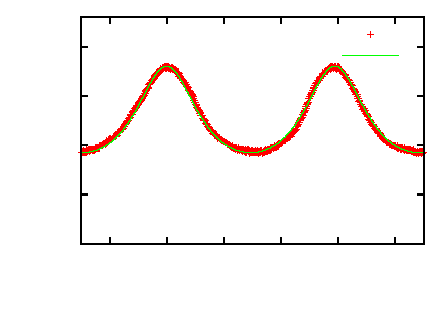
\includegraphics{finesse_messung_c}}%
    \gplfronttext
  \end{picture}%
\endgroup

		}
	}}
	\caption[Finesse des FPIs]{Die Abbildung zeigt die Plots des
 	Fringepattern für $772\,$nm (a), $633\,$nm (b) und $405\,$nm (c).}
	\label{fig:finesse_messung}
\end{figure}
Aus den Fits lassen sich die jeweiligen Reflektivitäten der Spiegel für die
Wellenlängen über
\begin{equation}\label{eq:finesse_messung_02}
	\begin{split}
		\kappa&=\frac{4R}{(1-R)^2}\\
		&\Leftrightarrow\\
		R&=\frac{2+\kappa-2\sqrt{1+\kappa}}{\kappa}
	\end{split}	
\end{equation}
berechnen. Tabelle \ref{tab:finesse} führt alle Reflektivitäten und Finessen
(nach \ref{eq:FPI_finesse}) auf. Wie schon in Abschn. \ref{sec:lasersystem}
erwähnt, hat das FPI im blauen Bereich eine sehr schlechte Finesse, mit der
allerdings immernoch gearbeitet werden kann. Im infraroten Bereich hat das FPI
offensichtlich die höchste Finesse.
\begin{table}[h]
	%Summe der Breiten muss 0.91 mal \textwidth sein.
	\begin{tabular}{C{0.40\textwidth}C{0.35\textwidth}C{0.16\textwidth}}
		\toprule
		\multicolumn{1}{C{0.05\textwidth}}{Wellenlänge [nm]} &
		\multicolumn{1}{C{0.15\textwidth}}{Spiegelreflektivität} &
		\multicolumn{1}{C{0.10\textwidth}}{Finesse}\\
		\midrule[1px]
		\hline
		%%%%%%%%%%%%%%%%%%%%%%%%%%%%%%%%%%%%%%%%%%%%%%%%%%%%%%%%%%%%%%%%%%%%%%
%%                                                                  %%
%%  This is a LaTeX2e table fragment exported from Gnumeric.        %%
%%                                                                  %%
%%%%%%%%%%%%%%%%%%%%%%%%%%%%%%%%%%%%%%%%%%%%%%%%%%%%%%%%%%%%%%%%%%%%%%
%Wellenlänge [nm]	&Spiegelreflektivität	&Finesse\\
772	&0,938	&49,47\\
633	&0,916	&35,79\\
405	&0,227	&1,936\\

		\bottomrule[1px]
	\end{tabular}
	\caption[FPI Finesse]{Aufgelistet sind die Messwerte für die Reflektivität der
	Spiegel und die Finesse des FPIs in Abhängigkeit von der Wellenlänge.}
	\label{tab:finesse}
\end{table}

\section{Stabilität der Laser}\label{sec:stabilitaet_der_laser}
Um die Lang- und Kurzzeitstabilität der Laser zu untersuchen wurden zwei
verschiedene Methoden angewandt. Zum einen wurde sowohl vom alten als auch vom
neuen Lasersystem das Frequenzverhalten mithilfe der neu entwickelte Software
aufgezeichnet. Zum anderen haben Schwebungsfrequenzmessungen zweier Laser mit
der nahezu gleichen Frequenz Relativfrequenzdaten beider Laser geliefert. Die
Ergebnisse dieser beiden Methoden sollen in diesem Abschnitt vorgestellt werden.

\subsection{Stabilitätsmessung mit neuer Software}
Das Frequenzverhalten aller drei Laser des neuen Systems wurde mit der neu
entwickelten Software über zwei Stunden hinweg analysiert, wobei die
Laser jeweils freilaufend, \textit{iScan}-stabilsiert und
\textit{iScan}+FOL-stabilisiert gemessen wurden. Weiterhin wurde das
Frequenzverhalten des Lasers für den zweiten Anregungsschritt aus dem alten Lasersystem mit der neuen Software aufgezeichnet,
während dieser mit der alten FOL-Technik stabilisiert wurde.\par
\begin{figure}[h]
 	\centering
 	\footnotesize
	% GNUPLOT: LaTeX picture with Postscript
\begingroup
  \makeatletter
  \providecommand\color[2][]{%
    \GenericError{(gnuplot) \space\space\space\@spaces}{%
      Package color not loaded in conjunction with
      terminal option `colourtext'%
    }{See the gnuplot documentation for explanation.%
    }{Either use 'blacktext' in gnuplot or load the package
      color.sty in LaTeX.}%
    \renewcommand\color[2][]{}%
  }%
  \providecommand\includegraphics[2][]{%
    \GenericError{(gnuplot) \space\space\space\@spaces}{%
      Package graphicx or graphics not loaded%
    }{See the gnuplot documentation for explanation.%
    }{The gnuplot epslatex terminal needs graphicx.sty or graphics.sty.}%
    \renewcommand\includegraphics[2][]{}%
  }%
  \providecommand\rotatebox[2]{#2}%
  \@ifundefined{ifGPcolor}{%
    \newif\ifGPcolor
    \GPcolortrue
  }{}%
  \@ifundefined{ifGPblacktext}{%
    \newif\ifGPblacktext
    \GPblacktexttrue
  }{}%
  % define a \g@addto@macro without @ in the name:
  \let\gplgaddtomacro\g@addto@macro
  % define empty templates for all commands taking text:
  \gdef\gplbacktext{}%
  \gdef\gplfronttext{}%
  \makeatother
  \ifGPblacktext
    % no textcolor at all
    \def\colorrgb#1{}%
    \def\colorgray#1{}%
  \else
    % gray or color?
    \ifGPcolor
      \def\colorrgb#1{\color[rgb]{#1}}%
      \def\colorgray#1{\color[gray]{#1}}%
      \expandafter\def\csname LTw\endcsname{\color{white}}%
      \expandafter\def\csname LTb\endcsname{\color{black}}%
      \expandafter\def\csname LTa\endcsname{\color{black}}%
      \expandafter\def\csname LT0\endcsname{\color[rgb]{1,0,0}}%
      \expandafter\def\csname LT1\endcsname{\color[rgb]{0,1,0}}%
      \expandafter\def\csname LT2\endcsname{\color[rgb]{0,0,1}}%
      \expandafter\def\csname LT3\endcsname{\color[rgb]{1,0,1}}%
      \expandafter\def\csname LT4\endcsname{\color[rgb]{0,1,1}}%
      \expandafter\def\csname LT5\endcsname{\color[rgb]{1,1,0}}%
      \expandafter\def\csname LT6\endcsname{\color[rgb]{0,0,0}}%
      \expandafter\def\csname LT7\endcsname{\color[rgb]{1,0.3,0}}%
      \expandafter\def\csname LT8\endcsname{\color[rgb]{0.5,0.5,0.5}}%
    \else
      % gray
      \def\colorrgb#1{\color{black}}%
      \def\colorgray#1{\color[gray]{#1}}%
      \expandafter\def\csname LTw\endcsname{\color{white}}%
      \expandafter\def\csname LTb\endcsname{\color{black}}%
      \expandafter\def\csname LTa\endcsname{\color{black}}%
      \expandafter\def\csname LT0\endcsname{\color{black}}%
      \expandafter\def\csname LT1\endcsname{\color{black}}%
      \expandafter\def\csname LT2\endcsname{\color{black}}%
      \expandafter\def\csname LT3\endcsname{\color{black}}%
      \expandafter\def\csname LT4\endcsname{\color{black}}%
      \expandafter\def\csname LT5\endcsname{\color{black}}%
      \expandafter\def\csname LT6\endcsname{\color{black}}%
      \expandafter\def\csname LT7\endcsname{\color{black}}%
      \expandafter\def\csname LT8\endcsname{\color{black}}%
    \fi
  \fi
  \setlength{\unitlength}{0.0500bp}%
  \begin{picture}(8502.00,6802.00)%
    \gplgaddtomacro\gplbacktext{%
      \csname LTb\endcsname%
      \put(1080,3401){\makebox(0,0)[r]{\strut{}-60}}%
      \put(1080,3796){\makebox(0,0)[r]{\strut{}-50}}%
      \put(1080,4191){\makebox(0,0)[r]{\strut{}-40}}%
      \put(1080,4586){\makebox(0,0)[r]{\strut{}-30}}%
      \put(1080,4981){\makebox(0,0)[r]{\strut{}-20}}%
      \put(1080,5376){\makebox(0,0)[r]{\strut{}-10}}%
      \put(1080,5771){\makebox(0,0)[r]{\strut{} 0}}%
      \put(1080,6166){\makebox(0,0)[r]{\strut{} 10}}%
      \put(1080,6561){\makebox(0,0)[r]{\strut{} 20}}%
      \put(1200,3201){\makebox(0,0){\strut{}}}%
      \put(2357,3201){\makebox(0,0){\strut{}}}%
      \put(3514,3201){\makebox(0,0){\strut{}}}%
      \put(4671,3201){\makebox(0,0){\strut{}}}%
      \put(5827,3201){\makebox(0,0){\strut{}}}%
      \put(6984,3201){\makebox(0,0){\strut{}}}%
      \put(8141,3201){\makebox(0,0){\strut{}}}%
      \put(500,4981){\rotatebox{-270}{\makebox(0,0){\strut{}relative Frequenz [MHz]}}}%
    }%
    \gplgaddtomacro\gplfronttext{%
      \csname LTb\endcsname%
      \put(5040,3964){\makebox(0,0)[r]{\strut{}freilaufend}}%
      \csname LTb\endcsname%
      \put(5040,3764){\makebox(0,0)[r]{\strut{}\textit{iScan}-stabilisiert}}%
      \csname LTb\endcsname%
      \put(5040,3564){\makebox(0,0)[r]{\strut{}\textit{iScan}+FOL-stabilisiert}}%
    }%
    \gplgaddtomacro\gplbacktext{%
      \csname LTb\endcsname%
      \put(1080,2585){\makebox(0,0)[r]{\strut{} 0.5}}%
      \put(1080,2791){\makebox(0,0)[r]{\strut{} 1}}%
      \put(1080,2996){\makebox(0,0)[r]{\strut{} 1.5}}%
      \put(1200,2180){\makebox(0,0){\strut{}}}%
      \put(2357,2180){\makebox(0,0){\strut{}}}%
      \put(3514,2180){\makebox(0,0){\strut{}}}%
      \put(4671,2180){\makebox(0,0){\strut{}}}%
      \put(5827,2180){\makebox(0,0){\strut{}}}%
      \put(6984,2180){\makebox(0,0){\strut{}}}%
      \put(8141,2180){\makebox(0,0){\strut{}}}%
    }%
    \gplgaddtomacro\gplfronttext{%
    }%
    \gplgaddtomacro\gplbacktext{%
      \csname LTb\endcsname%
      \put(1080,1615){\makebox(0,0)[r]{\strut{} 0.5}}%
      \put(1080,1870){\makebox(0,0)[r]{\strut{} 1}}%
      \put(1080,2125){\makebox(0,0)[r]{\strut{} 1.5}}%
      \put(1200,1160){\makebox(0,0){\strut{}}}%
      \put(2357,1160){\makebox(0,0){\strut{}}}%
      \put(3514,1160){\makebox(0,0){\strut{}}}%
      \put(4671,1160){\makebox(0,0){\strut{}}}%
      \put(5827,1160){\makebox(0,0){\strut{}}}%
      \put(6984,1160){\makebox(0,0){\strut{}}}%
      \put(8141,1160){\makebox(0,0){\strut{}}}%
      \put(500,1870){\rotatebox{-270}{\makebox(0,0){\strut{}Jitter [MHz]}}}%
    }%
    \gplgaddtomacro\gplfronttext{%
    }%
    \gplgaddtomacro\gplbacktext{%
      \csname LTb\endcsname%
      \put(1080,790){\makebox(0,0)[r]{\strut{} 0.5}}%
      \put(1080,980){\makebox(0,0)[r]{\strut{} 1}}%
      \put(1080,1170){\makebox(0,0)[r]{\strut{} 1.5}}%
      \put(1200,400){\makebox(0,0){\strut{}0}}%
      \put(2357,400){\makebox(0,0){\strut{}20}}%
      \put(3514,400){\makebox(0,0){\strut{}40}}%
      \put(4671,400){\makebox(0,0){\strut{}60}}%
      \put(5827,400){\makebox(0,0){\strut{}80}}%
      \put(6984,400){\makebox(0,0){\strut{}100}}%
      \put(8141,400){\makebox(0,0){\strut{}120}}%
      \put(4670,100){\makebox(0,0){\strut{}Zeit [min]}}%
    }%
    \gplgaddtomacro\gplfronttext{%
    }%
    \gplbacktext
    \put(0,0){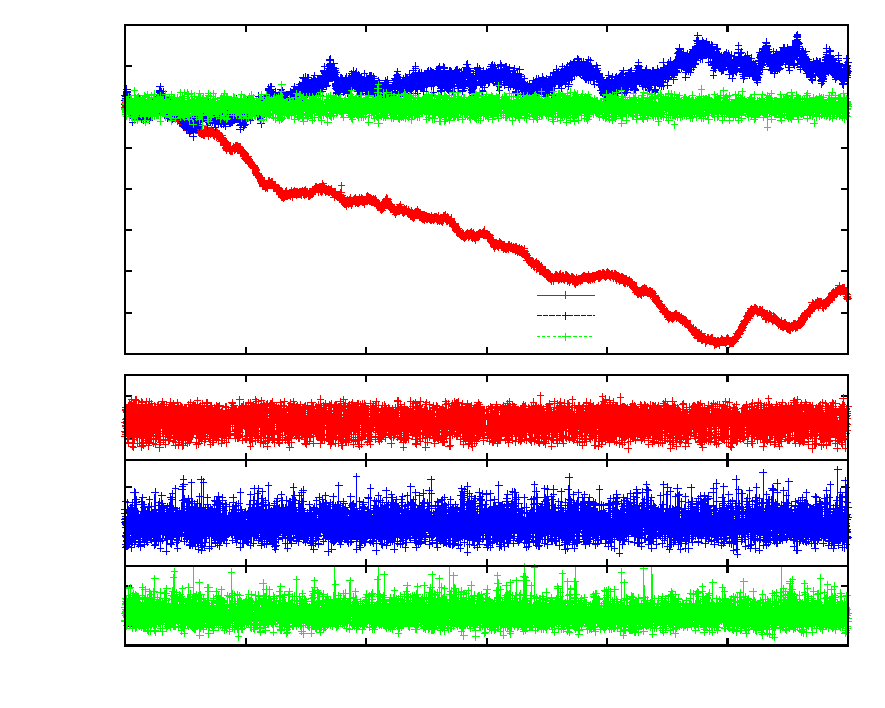
\includegraphics{laserstabilitaet_b_alles}}%
    \gplfronttext
  \end{picture}%
\endgroup

	\caption[Laserfrequenzverhalten \textit{DL-Pro}]{Die Abbildung zeigt das
	Laserfrequenzverhalten des \textit{DL-Pro} im freilaufenden (rot),
	\textit{iScan}-stabiliserten (blau) und \textit{iScan}+FOL-stabiliserten Modus
	(grün).
	Unten ist jeweils entsprechend farblich kodiert der Jitter aufgetragen.
	Separate, hochaufgelöstere Plots für alle Laser finden sich in Anh.
	\ref{anh:sec:laserstabilitaet}.}
	\label{fig:laserstabilitaet_b_alles}
\end{figure}
Abbildung \ref{fig:laserstabilitaet_b_alles} zeigt den relativen
Frequenzverlauf des \textit{DL-Pro} im freilaufenden (rot),
\textit{iScan}-stabiliserten (blau) und \textit{iScan}+FOL-stabiliserten Modus
(grün). Die Plots für die anderen beiden Laser befinden sich in Anh.
\ref{anh:sec:laserstabilitaet}. Sind die Laser nicht aktiv stabilisiert, driften
sie deutlich in der Frequenz. Der \textit{DL-Pro} driftet in zwei Stunden bis zu $60\,$MHz, wohingehen der
\textit{TA-Pro} nur einen maximalen Drift von $20\,$MHz vorweist. Dieser
Unterschied ist allerdings keine Systematik, da auch beim \textit{TA-Pro} schon
größere Drifts beobachtet wurden. Sehr viel größere Frequenzfluktuationen (bis $700\,$MHz)
weist der blaue Laser auf, was auf die wesentlich instabilere Mechanik
zurückzuführen ist. Größtenteils sind die Drift vermutlich mit der Temperatur
korreliert, was hier allerdings nicht nachgeprüft wurde. Eine weitere Ursache
ist der Piezoaktuator des Gitters, der nach Ändern der Spannung noch lange in
die gleiche Richtung nachdriftet. Der Jitter der Laser (Standardabweichung der
Frequenz über die durch den \textit{Arduino} gemittelten Werte) liegt für die
beiden \textit{Toptica}-Lasern bei maximal $1,5\,$MHz. Für den blauen Laser
liegt dieser bei etwa $5\,$MHz.\par
Wie erwartet reduziert sich der Drift bei \textit{iScan}-Stabilisierung,
verschwindet aber leider nicht völlig (immernoch ca. $20\,$MHz). Für den \textit{TA-Pro} ist die
\textit{iScan}-Stabilisierung kein besonderer Mehrgewinn, was allerdings wie
schon erwähnt nur speziell auf diese Messung zutreffend ist. Der blaue Laser
erfährt einen dramatischen Zugewinn an Stabilität mit einer Reduzierung des
Drifts auf ca. $100\,$MHz. Es zeigt sich, dass die \textit{iScans} zwar
eine hinreichend gute Stabilität in kurzen Zeitintervallen gewährleisten, jedoch
auf größeren Zeitskalen systematischen Schwankungen ausgeliefert sind. Die
wahrscheinlichste Ursache ist die sensible räumliche Abhängigkeit der
Einkopplung in die \textit{iScan heads}, was sich durch eine alternative
Faserkopplung überprüfen ließe. Eine weitere Ursache könnte trotz
Temperaturkontrolle die fehlende aktive Stabilisierung der internen \textit{iScan}-Optik sein. Der
Jitter ändert sich im Vergleich zum freilaufenden Fall nicht merklich, könnte
aber ggf. bei schlecht eingestelltem PID-Regler der \textit{iScans} etwas größer
sein, wie beim \textit{TA-Pro} zu erahnen ist.\par
%TODO: evtl. periodische Schwingung des Jitters erwähnen
Um die Drifts völlig zu eliminieren, muss das FOL hinzugeschaltet werden. Wie
Abb. \ref{fig:laserstabilitaet_b_alles} zeigt, reduziert sich
dank des FOL der Drift auf nahezu $0\,$MHz. Die Fluktuationen um die
Soll-Relativfrequenz (hier $0\,$MHz) ergibt sich nur noch aus dem Jitter der
Laser und der Regelung des FOL zu maximal $\pm12\,$MHz für den blauen und
$\pm4\,$MHz für die beiden roten Laser. Dieses Frequenzrauschen lässt sich ggf.
noch durch Variieren der Ober- und Untergrenzen für das FOL verkleinern, kann aber bei zu eng
gewählten Grenzen zu Überreglung und somit zu größeren Fluktuationen führen.\par
\begin{figure}[h]
 	\centering
 	\footnotesize
	% GNUPLOT: LaTeX picture with Postscript
\begingroup
  \makeatletter
  \providecommand\color[2][]{%
    \GenericError{(gnuplot) \space\space\space\@spaces}{%
      Package color not loaded in conjunction with
      terminal option `colourtext'%
    }{See the gnuplot documentation for explanation.%
    }{Either use 'blacktext' in gnuplot or load the package
      color.sty in LaTeX.}%
    \renewcommand\color[2][]{}%
  }%
  \providecommand\includegraphics[2][]{%
    \GenericError{(gnuplot) \space\space\space\@spaces}{%
      Package graphicx or graphics not loaded%
    }{See the gnuplot documentation for explanation.%
    }{The gnuplot epslatex terminal needs graphicx.sty or graphics.sty.}%
    \renewcommand\includegraphics[2][]{}%
  }%
  \providecommand\rotatebox[2]{#2}%
  \@ifundefined{ifGPcolor}{%
    \newif\ifGPcolor
    \GPcolortrue
  }{}%
  \@ifundefined{ifGPblacktext}{%
    \newif\ifGPblacktext
    \GPblacktexttrue
  }{}%
  % define a \g@addto@macro without @ in the name:
  \let\gplgaddtomacro\g@addto@macro
  % define empty templates for all commands taking text:
  \gdef\gplbacktext{}%
  \gdef\gplfronttext{}%
  \makeatother
  \ifGPblacktext
    % no textcolor at all
    \def\colorrgb#1{}%
    \def\colorgray#1{}%
  \else
    % gray or color?
    \ifGPcolor
      \def\colorrgb#1{\color[rgb]{#1}}%
      \def\colorgray#1{\color[gray]{#1}}%
      \expandafter\def\csname LTw\endcsname{\color{white}}%
      \expandafter\def\csname LTb\endcsname{\color{black}}%
      \expandafter\def\csname LTa\endcsname{\color{black}}%
      \expandafter\def\csname LT0\endcsname{\color[rgb]{1,0,0}}%
      \expandafter\def\csname LT1\endcsname{\color[rgb]{0,1,0}}%
      \expandafter\def\csname LT2\endcsname{\color[rgb]{0,0,1}}%
      \expandafter\def\csname LT3\endcsname{\color[rgb]{1,0,1}}%
      \expandafter\def\csname LT4\endcsname{\color[rgb]{0,1,1}}%
      \expandafter\def\csname LT5\endcsname{\color[rgb]{1,1,0}}%
      \expandafter\def\csname LT6\endcsname{\color[rgb]{0,0,0}}%
      \expandafter\def\csname LT7\endcsname{\color[rgb]{1,0.3,0}}%
      \expandafter\def\csname LT8\endcsname{\color[rgb]{0.5,0.5,0.5}}%
    \else
      % gray
      \def\colorrgb#1{\color{black}}%
      \def\colorgray#1{\color[gray]{#1}}%
      \expandafter\def\csname LTw\endcsname{\color{white}}%
      \expandafter\def\csname LTb\endcsname{\color{black}}%
      \expandafter\def\csname LTa\endcsname{\color{black}}%
      \expandafter\def\csname LT0\endcsname{\color{black}}%
      \expandafter\def\csname LT1\endcsname{\color{black}}%
      \expandafter\def\csname LT2\endcsname{\color{black}}%
      \expandafter\def\csname LT3\endcsname{\color{black}}%
      \expandafter\def\csname LT4\endcsname{\color{black}}%
      \expandafter\def\csname LT5\endcsname{\color{black}}%
      \expandafter\def\csname LT6\endcsname{\color{black}}%
      \expandafter\def\csname LT7\endcsname{\color{black}}%
      \expandafter\def\csname LT8\endcsname{\color{black}}%
    \fi
  \fi
  \setlength{\unitlength}{0.0500bp}%
  \begin{picture}(8502.00,6802.00)%
    \gplgaddtomacro\gplbacktext{%
      \csname LTb\endcsname%
      \put(1080,2380){\makebox(0,0)[r]{\strut{}-100}}%
      \put(1080,2977){\makebox(0,0)[r]{\strut{}-50}}%
      \put(1080,3575){\makebox(0,0)[r]{\strut{} 0}}%
      \put(1080,4172){\makebox(0,0)[r]{\strut{} 50}}%
      \put(1080,4769){\makebox(0,0)[r]{\strut{} 100}}%
      \put(1080,5366){\makebox(0,0)[r]{\strut{} 150}}%
      \put(1080,5964){\makebox(0,0)[r]{\strut{} 200}}%
      \put(1080,6561){\makebox(0,0)[r]{\strut{} 250}}%
      \put(1200,2180){\makebox(0,0){\strut{}}}%
      \put(2357,2180){\makebox(0,0){\strut{}}}%
      \put(3514,2180){\makebox(0,0){\strut{}}}%
      \put(4671,2180){\makebox(0,0){\strut{}}}%
      \put(5827,2180){\makebox(0,0){\strut{}}}%
      \put(6984,2180){\makebox(0,0){\strut{}}}%
      \put(8141,2180){\makebox(0,0){\strut{}}}%
      \put(380,4470){\rotatebox{-270}{\makebox(0,0){\strut{}relative Frequenz [MHz]}}}%
    }%
    \gplgaddtomacro\gplfronttext{%
      \csname LTb\endcsname%
      \put(3240,2743){\makebox(0,0)[r]{\strut{}freilaufend}}%
      \csname LTb\endcsname%
      \put(3240,2543){\makebox(0,0)[r]{\strut{}FOL-stabilisiert}}%
    }%
    \gplgaddtomacro\gplbacktext{%
      \csname LTb\endcsname%
      \put(1080,1565){\makebox(0,0)[r]{\strut{} 5}}%
      \put(1080,1770){\makebox(0,0)[r]{\strut{} 10}}%
      \put(1080,1975){\makebox(0,0)[r]{\strut{} 15}}%
      \put(1200,1160){\makebox(0,0){\strut{}}}%
      \put(2357,1160){\makebox(0,0){\strut{}}}%
      \put(3514,1160){\makebox(0,0){\strut{}}}%
      \put(4671,1160){\makebox(0,0){\strut{}}}%
      \put(5827,1160){\makebox(0,0){\strut{}}}%
      \put(6984,1160){\makebox(0,0){\strut{}}}%
      \put(8141,1160){\makebox(0,0){\strut{}}}%
      \put(500,1470){\rotatebox{-270}{\makebox(0,0){\strut{}Jitter [MHz]}}}%
    }%
    \gplgaddtomacro\gplfronttext{%
    }%
    \gplgaddtomacro\gplbacktext{%
      \csname LTb\endcsname%
      \put(1080,790){\makebox(0,0)[r]{\strut{} 5}}%
      \put(1080,980){\makebox(0,0)[r]{\strut{} 10}}%
      \put(1080,1170){\makebox(0,0)[r]{\strut{} 15}}%
      \put(1200,400){\makebox(0,0){\strut{}0}}%
      \put(2357,400){\makebox(0,0){\strut{}20}}%
      \put(3514,400){\makebox(0,0){\strut{}40}}%
      \put(4671,400){\makebox(0,0){\strut{}60}}%
      \put(5827,400){\makebox(0,0){\strut{}80}}%
      \put(6984,400){\makebox(0,0){\strut{}100}}%
      \put(8141,400){\makebox(0,0){\strut{}120}}%
      \put(4670,100){\makebox(0,0){\strut{}Zeit [min]}}%
    }%
    \gplgaddtomacro\gplfronttext{%
    }%
    \gplbacktext
    \put(0,0){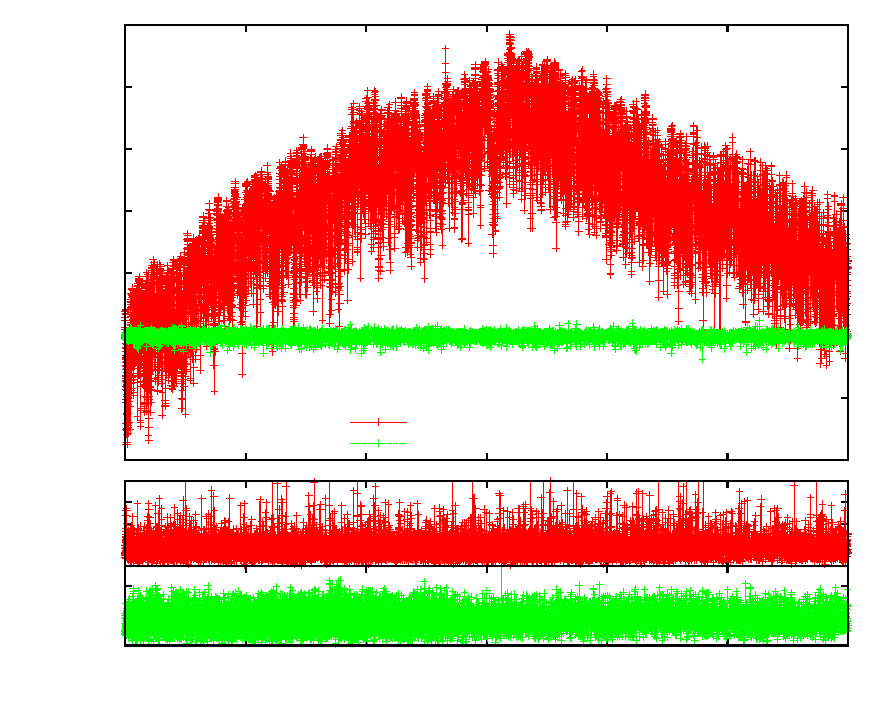
\includegraphics{laserstabilitaet_alt_alles}}%
    \gplfronttext
  \end{picture}%
\endgroup

	\caption[Laserfrequenzverhalten altes System]{Die Abbildung zeigt das
	Frequenzverhalten des Lasers für den zweiten Anregungsschritts im alten System
	im freilaufenden (rot) und FOL-stabiliserten Modus (grün).
	Unten ist jeweils in des entsprechenden Farben der Jitter aufgetragen.
	Separate, hochaufgelöstere Plots hierfür finden sich in Anh.
	\ref{anh:sec:laserstabilitaet}.}
	\label{fig:laserstabilitaet_alt_alles}
\end{figure}
Abbildung \ref{fig:laserstabilitaet_alt_alles} zeigt die Plots für den
roten Laser des zweiten Anregungsschritts im alten System, dessen Daten auch über zwei Stunden aber mit einer
höreren Rate\footnote{Die Daten wurden zu einem Zeitpunkt aufgenommen, an dem die Software schon in einem performanteren
Stadium war und mit einer höheren Rate Laserdaten verarbeiten konnte.}
aufgenommen wurden (rot: freilaufend;
grün: FOL-stabilisiert). Seperate, hochaufgelöstere Plots finden sich im Anh.
\ref{anh:sec:laserstabilitaet}. Im freilaufenden Modus driftet der Laser bis
zu $300\,$MHz in zwei Stunden. Der Jitter liegt bei etwa $5\,$MHz, wurde
aber auf der Grundlage weniger Rampenzyklen berechnet und muss deshalb in der
Größenordnung von $100\,$ms angesiedelt werden. Es zeigt sich, dass die
Frequenzfluktuation darüber hinaus aber in der Größenordnung von mehreren
Sekunden gut $100\,$MHz beträgt, was normalerweise für die Laser dieser Bauart
nicht üblich ist. Ein möglicher Grund können Schwebungen von Vibrationen sein,
die beispielsweise durch die Vorpumpe der Vakuumaparatur ausgelöst werden. Im
stabilisierten Modus zeigt der Laser ein vergleichbares Verhalten mit
dem blauen Laser aus dem neuen System, was aufgrund der gleichen Bauart nicht
verwunderlich ist. Der Jitter fluktuiert hier scheinbar mehr als beim blauen
Laser. Dies liegt aber daran, dass hier seitens des \textit{Arduinos} über
wesentlich weniger Werte gemittelt wurde. Auch verschindet erfreulicherweise der
makroskopische Jitter.\par
In der Effizienz der aktiven Stabilisierung unterscheiden sich die beiden
Lasersysteme also nicht merklich. Der einzige offensichtliche Vorteil des neuen
Systems liegt in der Bauweise der \textit{Toptica}-Laser, die die
Grundstabilität enorm steigert. Fluktuationen wie im Falle des Lasers aus dem
alten System werden somit von Grund auf unterdrückt.

\subsection{Stabilitätsmessung über
Schwebungsfrequenzen}\label{subsec:beatfrequenzmessung}
Um die Messungen im vorherigen Abschnitt durch eine wesentlich direktere
Methode zur Relativfrequenzanalyse zu bestärken, eignet sich hervorragend die
Messung von Schwebungsfrequenzen der beiden roten Laser. Dazu wurden wie in Abb.
\ref{fig:beatfrequenzmessung_aufbau_schematisch} schematisch dargestellt jeweils
ein Teilstrahl der beiden Laser über einen Polarisationsstrahlteiler
überlagert und auf eine Photodiode geschickt. Bringt man nun die Frequenzen
beider Laser auf sehr nahe beieinander liegende Frequenzen (wenige MHz
Unterschied), entsteht durch Interferenz beider
elektromagnetischen Felder ein Schwebungssignal mit der Differenzfrequenz
(siehe Abb. \ref{fig:schwebungssignal}), welches über den Strom der Photodiode
an einem Oszilloskop spektral analysiert werden kann.
Sowohl für das neue als auch für das neue System wurden bei
stabilisierten Lasern Schwebungssignale analysiert. Beim neuen System wurde
zwischen der Stabilisierung nur mit \textit{iScans} und der Kombination von
\textit{iScan} und 
